\documentclass{InsightArticle}

\usepackage[dvips]{graphicx}
\usepackage{float}
\usepackage{subfigure}

\usepackage[dvips,
bookmarks,
bookmarksopen,
backref,
colorlinks,linkcolor={blue},citecolor={blue},urlcolor={blue},
]{hyperref}

\title{Interactive Image Graph Cut Segmentation}

% 
% NOTE: This is the last number of the "handle" URL that 
% The Insight Journal assigns to your paper as part of the
% submission process. Please replace the number "1338" with
% the actual handle number that you get assigned.
%
\newcommand{\IJhandlerIDnumber}{3233}

% Increment the release number whenever significant changes are made.
% The author and/or editor can define 'significant' however they like.
\release{0.00}

% At minimum, give your name and an email address.  You can include a
% snail-mail address if you like.

\author{David Doria, Siqi Chen}
\authoraddress{Rensselaer Polytechnic Institute, Troy NY}


\begin{document}

\IJhandlefooter{\IJhandlerIDnumber}


\ifpdf
\else
   %
   % Commands for including Graphics when using latex
   % 
   \DeclareGraphicsExtensions{.eps,.jpg,.gif,.tiff,.bmp,.png}
   \DeclareGraphicsRule{.jpg}{eps}{.jpg.bb}{`convert #1 eps:-}
   \DeclareGraphicsRule{.gif}{eps}{.gif.bb}{`convert #1 eps:-}
   \DeclareGraphicsRule{.tiff}{eps}{.tiff.bb}{`convert #1 eps:-}
   \DeclareGraphicsRule{.bmp}{eps}{.bmp.bb}{`convert #1 eps:-}
   \DeclareGraphicsRule{.png}{eps}{.png.bb}{`convert #1 eps:-}
\fi


\maketitle


\ifhtml
\chapter*{Front Matter\label{front}}
\fi

\begin{abstract}
\noindent
This document presents a system to ``scribble`` on an image to mark foreground and background pixels and then feed these pixels to a graph cuts segmentation technique. The interaction is done using the Visualization Toolkit and the processing is done using the Insight Toolkit. The graph cut function itself is the maxflow-v2.21 algorithm written by Yuri Boykov and Vladimir Kolmogorov. This version of their algorithm is released under a GPL license.

\end{abstract}

\IJhandlenote{\IJhandlerIDnumber}

\tableofcontents
\section{Introduction}
Automatic image segmentation algorithms are constantly improving. However, the best results can still be obtained by requiring human input and feedback throughout the segmentation process. This system allows the user to indicate foreground and background pixels using a ``scribble'' technique. The segmentation result can be iteratively refined and recomputed until the desired segmentation is obtained.

We have implemented the algorithm described in \cite{boykov2006}. The basic workflow is:
\begin{itemize}
\item ``Scribble'' to select foreground and background pixels
\item Set $\lambda$
\item Perform the segmentation
\item Iteratively refine
\end{itemize}

Our implementation can operate on images with arbitrary pixel types. That is, we can operate on grayscale images, RGB images, or N-D images, each with components of any scalar type.

%%%%%%%%%%%%%%%%
\section{Segmentation Algorithm}
\label{sec:Algorithm}
As described in \cite{boykov2006}, the energy function to be minimized is
\begin{equation}
 E(A) = \lambda R(A) + B(A)
\end{equation}
where $A$ is a linearized vector of pixel assignments (foreground or background), $R(A)$ is the regional term (see Section \ref{subsec:RegionalTerm}) and $B(A)$ is the boundary term (see Section \ref{subsec:BoundaryTerm}).

\subsection{Regional Term}
\label{subsec:RegionalTerm}
\begin{equation}
 R(A) = \sum_{p \in P} R_p(A_p)
\end{equation}

As suggested in \cite{boykov2006}, we have used
\begin{equation}
 R_p(object) = -ln Pr(I_p|object)
\end{equation}
\begin{equation}
 R_p(background) = -ln Pr(I_p|background)
\end{equation}

which reflect how the intensity of pixel $p$ fits the histogram of the foreground and background models.

\subsection{Boundary Term}
\label{subsec:BoundaryTerm}
The boundary term and is described by:
\begin{equation}
 B(A) = \sum_{ \{p,q\} \in N} B_{p,q} \delta_{A_p\neq A_q}
\end{equation}

where 
\begin{equation*}
\delta_{A_p\neq A_q} =
\begin{cases} 
1 & \text{if } A_p = A_q
\\
0 & otherwise
\end{cases}
\end{equation*}

The choice of $B_{p,q}$ is taken to be:
\begin{equation}
 B_{p,q} \propto \exp\left(-\frac{(I_p - I_q)^2}{2\sigma^2}\right) \frac{1}{dist(p,q)}
\end{equation}

Since we have used a 4-connected neighborhood, $dist(p,q)$ is always equal to $1$.

\subsection{General Behavior}
When $\lambda$ is high, there is no regularization. That it, each pixel decides if it belongs to the foreground or background based only on its color (without looking at its neighbors). Another way to say this is that the segmentation problem degenerates into a clustering problem. If $\lambda$ is set to $0$, only the boundary term is considered. This scenario produces a trivial solution, so we produce an error if the user specifies this condition.

%%%%%%%%%%%%%%%
\section{Implementation Details}
\subsection{Structure}
Our code has three main components: 
\begin{itemize}
\item The GUI (GraphCutSegmentationWidget.h, GraphCutSegmentationWidget.cpp, GraphCutSegmentationWidget.ui)
\item The ``scribbling'' code (in a submodule called ScribbleInteractorStyle)
\item The graph cut segmentation code (in a submodule called ImageGraphCutSegmentation)
\end{itemize}
 
\subsection{GUI}
\label{subsec:GUI}
We used Qt for our GUI. The window is split into two main components. The left side is the input image, and the right side is the output (segmented) image.
\subsubsection{Input Image}
On the left of the form, the input image is displayed. Below the input image are radio buttons to chose whether the scribbling will select foreground or background pixels. A ``Clear Selections'' button is provided to allow the user to start over at any point.
\subsubsection{Segmented (Output) Image}
\paragraph{Lambda}
On the right of the form, a window is provided to view the result of the segmentation. Below this window, the segmentation parameters can be set. Lambda ($\lambda$) controls the relative proportion of the Regional Term in the energy function. Setting $\lambda = 0$ makes the energy function exactly equal to the Boundary Term only. We provide a combination of a slider and a text box to set $\lambda$. The text box allows the user to specify the maximum $\lambda$. The the slider sets the percentage of the maximum $\lambda$ to actually use as $\lambda$ in the graph construction.

\paragraph{Number Of Histogram Bins}
A slider allows the user to set the $NumberOfHistogramBins$ to use when constructing the foreground and background histograms.

\subsection{Scribbling}
To perform the scribbling, we use a vtkImageTracerWidget under the hood. Foreground scribbles are displayed in green while background scribbles are displayed in red. The vtkInteractorStyleScribble contains the vtkImageTracerWidget and provides the GraphCutSegmentationWidget with the scribbles that the user has input. We convert the list of points in the vtkPolyData returned by the vtkImageTracerWidget into a
\begin{verbatim}
std::vector<itk::Index<2> > 
\end{verbatim}

for both the Sources and Sinks (members of the ImageGraphCutBase). Since the vtkImageTracerWidget operates in a real coordinate space (non-discrete, non-pixel space), and does not guarantee a particular spacing of the points on the curve, we compute Bresenham lines between all adjacent points in the (ordered) list of points from the tracer to produce the list of pixels that lie under the stroke.

\subsection{ImageGraphCut}
The function of this class is to create the graph which will be fed to Kolmogorov's S-T min-cut implementation. The structure of the graph is a uniform (regular) grid of 4-connected nodes (the pixels). The edge weights between these nodes are called ``n-weighs''.  Additionally, each pixel is connected to both a synthetic foreground node and a synthetic background node. Each of these edges is weighted with a ``t-weight''.

\subsection{ImageGraphCutBase and ImageGraphCut}
We want the segmentation to work for images of arbitrary pixel type. To allow for this, we want to template ImageGraphCut on the type of image to be segmented. However, we want to allow the user to specify this type at runtime. Therefore, we must store (in the Form class) a pointer to a base class of ImageGraphCut so that we can instantiate the ImageGraphCut template with the appropriate type when necessary.

\subsubsection{ImageGraphCutBase}
This class contains all of the functions which are not type-dependent. Its main purpose is to allow us to do the following in the Form class:
\begin{verbatim}
ImageGraphCutBase* GraphCut;

// ... later ...

this->GraphCut = new ImageGraphCut<TImageType>(reader->GetOutput());
\end{verbatim}

\subsubsection{ImageGraphCut}
This class contains all of the type-dependent functions. It is here that we create the graph (CreateGraph()) and cut the graph (CutGraph()). In ImageGraphCut we also compute the histograms which are used in the Region Term computation (as shown in Section \ref{subsec:RegionalTerm}).

\subsection{Creating the Nodes}
Kolmogorov's S-T implementation requires each node ID to be stored as a \verb|void*|. To keep track of this, we create an image of type:
\begin{verbatim}
typedef itk::Image<void*, 2> NodeImageType;
\end{verbatim}

of the same size as the input image. We add all of nodes to the Graph object while storing their IDs in a NodeImage. This implicitly maintains the mapping from pixel index to node ID.

\begin{verbatim}
// Add all of the nodes to the graph and store their IDs in a "node image"
itk::ImageRegionIterator<NodeImageType> nodeImageIterator(this->NodeImage, this->NodeImage->GetLargestPossibleRegion());
nodeImageIterator.GoToBegin();

while(!nodeImageIterator.IsAtEnd())
  {
  nodeImageIterator.Set(this->Graph->add_node());
  ++nodeImageIterator;
  }
\end{verbatim}


\subsubsection{N-Weights}
The N-weight are computed using the procedure described in Section \ref{subsec:BoundaryTerm}.

\begin{verbatim}
float pixelDifference = PixelDifference(centerPixel, neighborPixel);
float weight = exp(-pow(pixelDifference,2)/(2.0*sigma*sigma));

void* node1 = this->NodeImage->GetPixel(iterator.GetIndex(center));
void* node2 = this->NodeImage->GetPixel(iterator.GetIndex(neighbors[i]));
this->Graph->add_edge(node1, node2, weight, weight);
\end{verbatim}

\subsubsection{Histograms}
We use itkSampleToHistogramFilter to create a histogram of the selected foreground pixels (ForegoundHistogram) and background pixels (BackgroundHistogram). The dimensionality of the histogram is determined by the dimensionality of the input image pixel type. A parameter, $NumberOfHistogramBins$, controls the granularity of the histograms. If the user has selected to open the image as a color image (from the File menu), a 3D histogram (R, G, B) is computed and used. If the user has selected to open the image as a grayscale image, a 1D histogram (gray value) is used.

\subsubsection{T-Weights}
The synthetic foreground and background nodes are automatically created by Kolmogorov's implementation. We simply must set the edge weight from every N-node we have created to both the synthetic foreground (source) and synthetic background (sink) nodes. The weights as computed as described in Section \ref{subsec:RegionalTerm}.

\begin{verbatim}
this->Graph->add_tweights(nodeIterator.Get(),
                          -this->Lambda*log(sinkHistogramValue),
                          -this->Lambda*log(sourceHistogramValue));
\end{verbatim}
(Note: $log()$ is the natural log in c++).

The nodes which were directly specified by the user via scribbling are set to definitely belong to the corresponding synthetic node by setting the weight for node it belongs to to \verb|std::numeric_limits<float>::max()| and the node it does not belong to to $0$. This translates to ``you cannot cut this edge'' and ``there is no cost for cutting this edge'', respectively. We must use \verb|max()| rather than \verb|infinity()| because if $\lambda$ is zero, the weight should be zero, and \verb|0 *  std::numeric_limits<float>::infinity()| is NaN.

%%%%%%%%%%%%%%%
\section{Screenshots}
\subsection{Basic Environment}
Figure \ref{fig:Environment} shows the GUI as described in Section \ref{subsec:GUI}.

\begin{center}
	\begin{figure}[H]
  \centering
		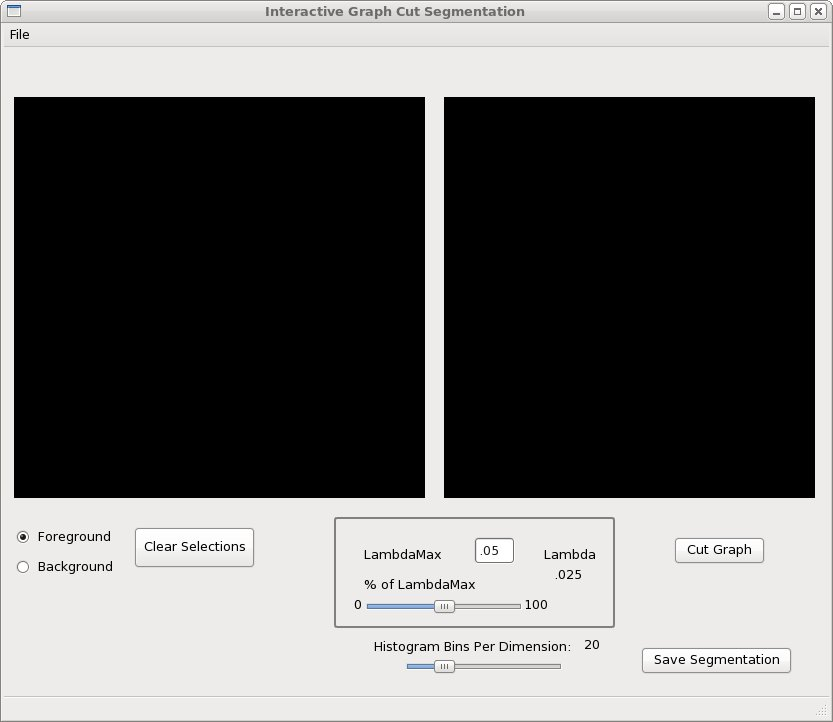
\includegraphics[width=0.6\linewidth]{images/Environment}
		\caption{Default Environment}
		\label{fig:Environment}
	\end{figure}
\end{center} 

\subsection{Scribbling}

Figure \ref{fig:Scribbling} shows the GUI after the user has scribbled to select both foreground (green) and background (red) pixels.

\begin{center}
	\begin{figure}[H]
  \centering
		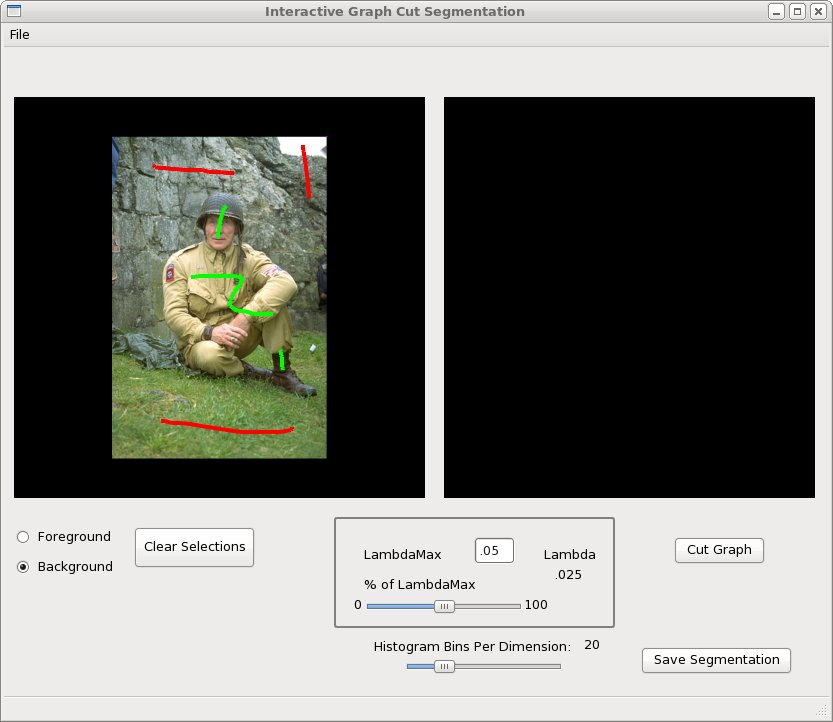
\includegraphics[width=0.6\linewidth]{images/Scribbling}
		\caption{Scribbling}
		\label{fig:Scribbling}
	\end{figure}
\end{center} 

\subsection{Simple Example Image}
A simple example image from the Berkeley Segmentation Dataset (http://www.eecs.berkeley.edu/Research/Projects/CS/vision/grouping/segbench/) is used for demonstrative purposes.

Figure \ref{fig:HighLambda} shows the resulting segmentation when $\lambda$ is too high. Notice that many non-contiguous pixels are incorrectly considered to be in the foreground on the basis of their color only (the lines of shadows are closer to the dark colored sand than the light colored sand).

\begin{center}
	\begin{figure}[H]
  \centering
		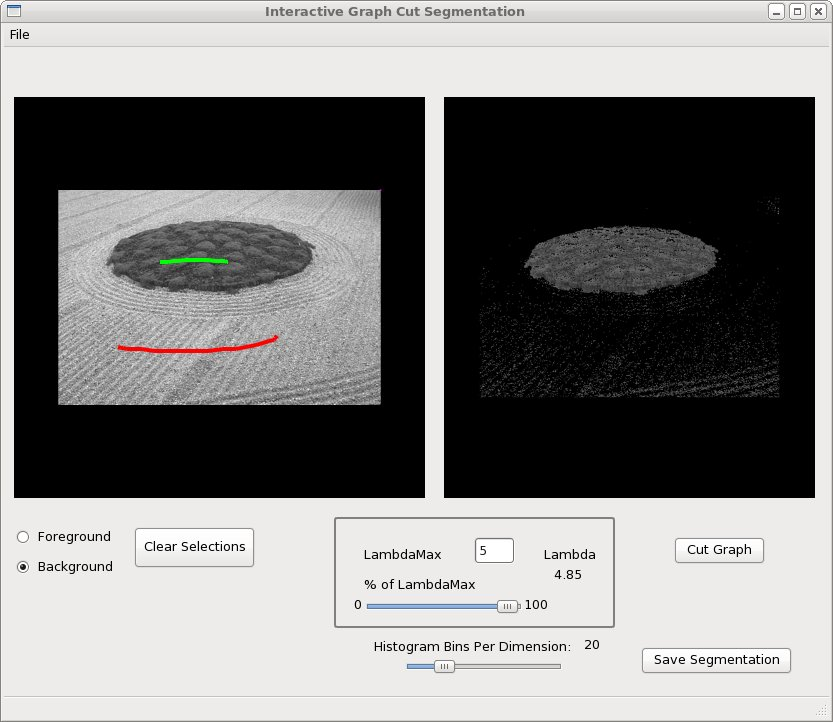
\includegraphics[width=0.6\linewidth]{images/HighLambda}
		\caption{Result of grayscale segmentation of Sand image with $\lambda$ set too high.}
		\label{fig:HighLambda}
	\end{figure}
\end{center} 

Figure \ref{fig:Sand} shows the resulting segmentation when $\lambda$ is set properly. This choice of $\lambda$ puts enough weight on the Region Term to encourage a very connected segmentation.

\begin{center}
	\begin{figure}[H]
  \centering
		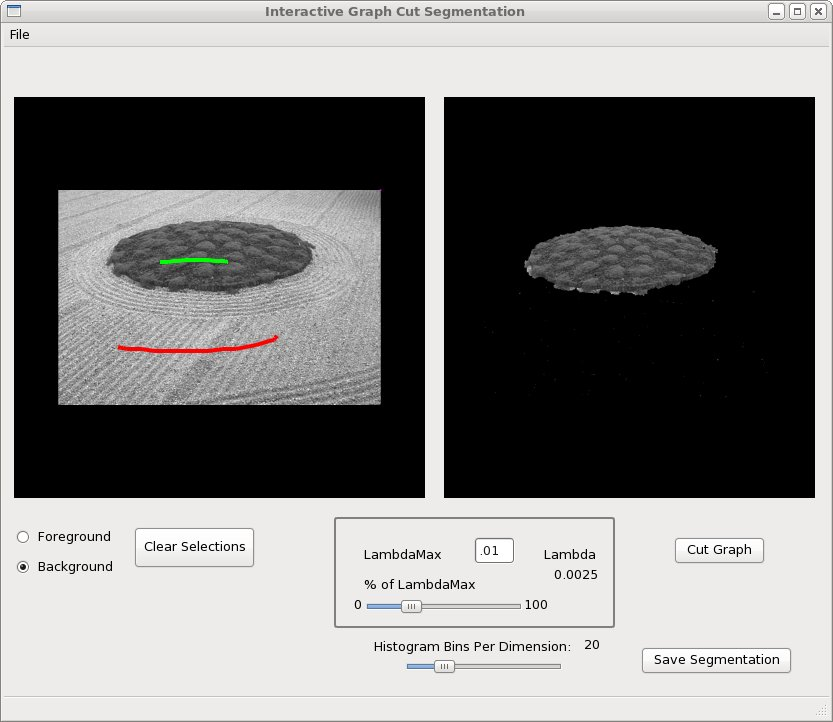
\includegraphics[width=0.6\linewidth]{images/Sand}
		\caption{Result of grayscale segmentation of Sand image with $\lambda$ set properly.}
		\label{fig:Sand}
	\end{figure}
\end{center} 

\subsection{Difficult Image}
To show that this does not just work in trivial cases, we show the result of the segmentation of a difficult image in Figure \ref{fig:Soldier}.

\begin{center}
	\begin{figure}[H]
  \centering
		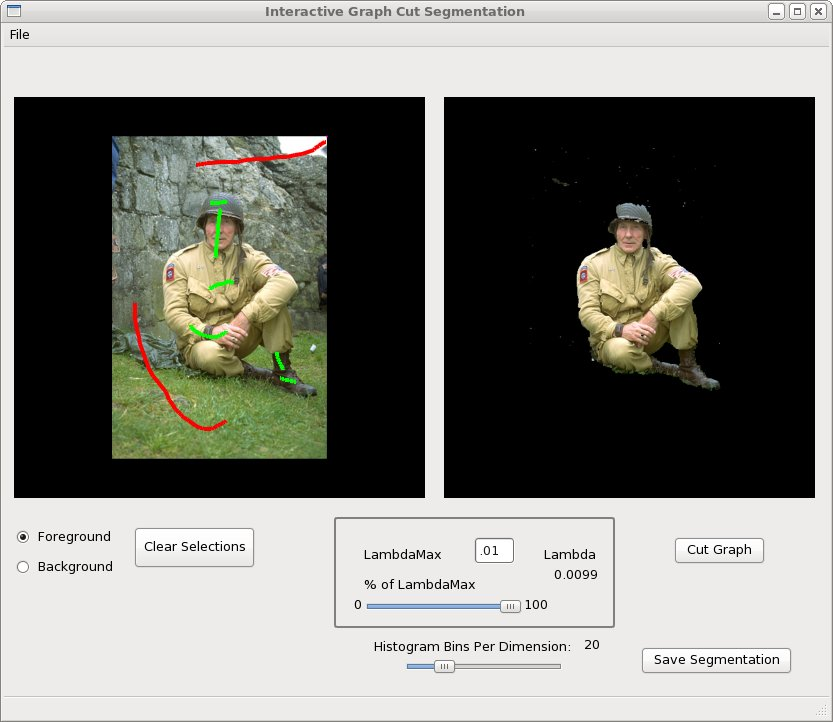
\includegraphics[width=0.6\linewidth]{images/Soldier}
		\caption{Result of color segmentation of Soldier image.}
		\label{fig:Soldier}
	\end{figure}
\end{center} 

%%%%%%%%%%%%%%%
\begin{thebibliography}{9}

	\bibitem{boykov2006}
	  Yuri Boykov,
	  \emph{Graph Cuts and Efficient N-D Image Segmentation}.
	  International Journal of Computer Vision
	  2006

\end{thebibliography}

\end{document}